\documentclass{article}% option leqno pour aligner les numéros d'équations à gauche
                                    % option fleqn pour aligne les équations à gauche

\usepackage[utf8]{inputenc}%          encodage en utf8 du fichier soruce
\usepackage[T1]{fontenc}%             encodage de police pour gérer les accents français
\usepackage[francais]{babel}%         documen en langue française uniquement
\usepackage{textcomp}%                caractères additionnels
\usepackage{amsmath,amssymb,amsthm}%  packages de l'AMS
\usepackage{txfonts}%                 pour utilsier la police times
\usepackage[a4paper]{geometry}%       pour gérer la taille du papier et les marges
\usepackage{graphicx}%                pour inclure des images
\usepackage{xcolor}%                  pour gérer les couleurs
\usepackage{microtype}%               diverses améliorations typographiques

\usepackage[Algorithme]{algorithm}
\usepackage{algorithmic}
\usepackage{listings}

\usepackage{wrapfig}%                 pour mettre des images dans le texte

\usepackage{titling}%                 pour personnaliser le titre
\usepackage[runin]{abstract}%         pour personnaliser l'abstract ; l'option runin ne met pas le titre au-dessus
%\usepackage{titlesec}%                pour personnaliser les sections
\usepackage{titletoc}%                pour personnaliser la table des matières
\usepackage{fancyhdr}%                pour personnaliser les en-têtes et pieds de pages
\usepackage{footmisc}%                pour personnaliser les footnotes

\usepackage{hyperref}%                gestion des hyperliens --> À METTRE EN DERNIER
\hypersetup{pdfstartview=XYZ}%        restauration du zoom par défaut


% PERSONNALISATION DE LA PAGE
% marges
\geometry{top=3cm,bottom=2.5cm}


% PERSONNALISATION DU TITRE AVEC TITLING
% au-dessus du titre
\setlength{\droptitle}{-1cm}
\renewcommand{\maketitlehooka}{{\setlength{\parindent}{0cm}\scriptsize
  \emph{Master 2 Algèbre Appliquées} \hfill Projet étudiant

  Université Paris-Saclay \hfill Algorithmique et programmation C
  
  2016 - 2017 \hfill MIT Licence
  
  \vspace{1cm}
}}
% titre
\pretitle{\begin{center}\large\bfseries\MakeUppercase}
\posttitle{\par\rule{5cm}{0.56pt}\end{center}}
% auteur
\preauthor{\begin{center}
  \textit{par} \scshape \lineskip 0.5em%
}
\postauthor{\par\end{center}}
\renewcommand{\and}{\unskip, }% parce qu'on a supprimé le tableau
% date
\predate{\begin{center}\small le }
%\postdate{\par\end{center}\vspace{1cm}}


% PERSONNALISATION DU RÉSUMÉ AVEC LE PACKAGE ABSTRACT
\renewcommand{\abstractnamefont}{\normalfont\small\scshape}
\abslabeldelim{. ---}
\setlength{\absleftindent}{\parindent}
\setlength{\absrightindent}{\parindent}
\setlength{\abstitleskip}{-\parindent}


% PERSONNALISATION DES THÉORÈMES
% théorèmes
\newtheoremstyle{plain}
  {\topsep}%   espacement avant le théorème
  {\topsep}%   espacement après le théorème
  {\itshape}%  police du corps du théorème
  {}%          indentation (vide pour aucune indentation, sinon \parindent ou une autre longueur)
  {\scshape}%  police du titre du théorème  
  {}%     ponctuation après le titre du théorème
  {\newline}%         espace après le titre du théorème (soit une espace, soit une longueur soit un \newline)
  {\llap{}\thmname{#1}\thmnumber{ #2}\thmnote{ \normalfont(#3)}}% spécification du titre
\theoremstyle{plain}
\newtheorem{theoreme}{Théorème}[section]
\renewcommand{\thetheoreme}{\thesection.\textsc{\roman{theoreme}}}

% définition
\theoremstyle{definition}
\newtheorem{definition}{Définition}[section]


% proposition
\theoremstyle{plain}
\newtheorem{proposition}{Proposition}[section]

% corollaire
\theoremstyle{plain}
\newtheorem{corollaire}{Corollaire}[section]

% remarque
\newtheoremstyle{remark}
  {\topsep}%   space before
  {\topsep}%   space after
  {}%  Body font
  {}%          Indent amount (empty for no indent, \parindent)
  {\itshape}% Thm head font   
  {. ---}%         Punctuation after thm head
  { }%         Space after thm head (\newline = linebreak)
  {\thmname{#1}\thmnumber{ #2}\thmnote{ \normalfont(#3)}}% Thm head spec
\theoremstyle{remark}
\newtheorem*{remarque}{Remarque}





% PERSONNALISATION DE LA TABLE DES MATIÈRES AVEC LE PACKAGE TITLETOC
\addto\captionsfrench{\renewcommand{\contentsname}{Sommaire}}
%\contentsmargin{2em}% il faut augmenter la largeur de \contentspage car les numéros de pages ont 3 chiffres
\titlecontents{section}
  [0pc]
  {}
  {§~\thecontentslabel.~}
  {}
  {\titlerule*[0.75em]{.}\contentspage}
 \titlecontents{subsection}
  [0pc]
  {}
  {§~\thecontentslabel.~}
  {}
  {\titlerule*[0.75em]{.}\contentspage}


% PERSONNALISATION DES NUMÉROS DE PAGE
%\setcounter{page}{356}


% PERSONNALISATION DES EN-TÊTES AVEC LE PACKAGE FANCYHDR
\pagestyle{fancy}
\fancyhead{}
\makeatletter
\fancyhead[R]{\itshape\@title}
\makeatother
\fancyhead[L]{\scshape\theauthor}
\renewcommand{\headrulewidth}{0pt}


% PERSONNALISATION DES NUMÉROS D'ÉQUATION
%\numberwithin{equation}{section}
%\renewcommand{\theequation}{\thesection.\textit{\alph{equation}}}


% PERSONNALISATION DES FOOTNOTE AVEC LE PACKAGE FOOTMISC
% numérotation en \fnsymbol des footnotes
\renewcommand{\thefootnote}{\fnsymbol{footnote}}
% utilisation de footmisc pour redéfinir \fnsymbol
\DefineFNsymbols*{daggers}{%
  {\textdagger}%
  {\textdaggerdbl}%
  {\textdagger\textdagger}%
  {\textdaggerdbl\textdaggerdbl}%
  {\textdagger\textdagger\textdagger}%
  {\textdaggerdbl\textdaggerdbl\textdaggerdbl}%
  {\textdagger\textdagger\textdagger\textdagger}%
  {\textdaggerdbl\textdaggerdbl\textdaggerdbl\textdaggerdbl}%
}
\setfnsymbol{daggers}
% désactivation de babel pour l'apparence de la footnote en bas de la page
\frenchbsetup{FrenchFootnotes=false}


% TITRE DU DOCUMENT
\title{Comptage de points d'une courbe elliptique sur des corps finis}
\author{Daniel RESENDE\\supervisé par Luca DE FEO}
\date{\today}

\newcommand\fq{\mathbf{F}_{q}}
\newcommand\ie{\textit{i.e.}}

\begin{document}

\maketitle

\begin{abstract}
Il s'agit de la description de l'algorithme de René Schoof. Celui-ci fût le premier algorithme de comptage de points d'une courbe elliptique sur des corps finis en un temps polynomial ($O(\log^{9} p)$).  
\end{abstract}

\tableofcontents

\clearpage\addcontentsline{toc}{section}{Introduction}
\section*{Introduction}

\begin{wrapfigure}{r}{0cm}
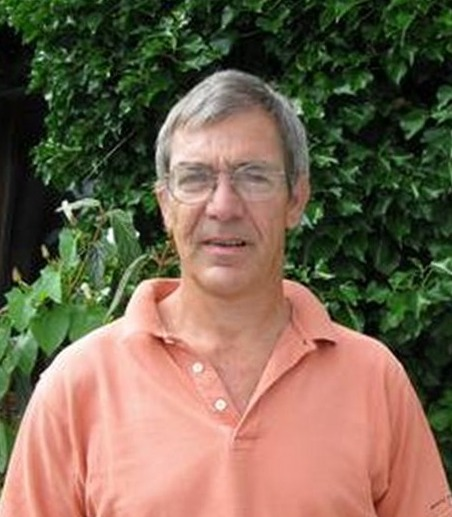
\includegraphics[width=3cm]{Rene_Schoof.jpg}
\caption{\label{étiquette}Portrait René Schoof}
\end{wrapfigure}
Les courbes elliptiques définissent une loi de groupe sur les corps finis $\fq$ qui est difficile pour le problème du logarithme discret. On retrouve par conséquent son utilisation dans plusieurs schémas cryptographiques comme Diffie-Hellman (avec ECDH) ou El-Gamal (avec ECDSA).
Cependant, l'utilisation de schémas à l'aide de courbes elliptiques nécessite d'avoir un grand nombre premier qui divise l'ordre d'un sous-groupe cyclique de $E(\fq)$. Nous avons donc besoin de connaitre le cardinal de $E(\fq)$.

\begin{list}{•}{Il existe aujourd'hui de nombres algorithme de comptage de points d'une courbes elliptiques sur un corps finis $\fq$ :}
\item L'algorithme de Shank en 1971 basé sur Baby Step Giant Step et le théorème de Hasse,
\item L'algorithme Schoof en 1985 que l'on va étudier dans ce mémoire,
\item L'algorithme SEA [Schoof, Elkies, Atkin] en 1995 qui est une amélioration de l'algorithme de Schoof,
\item L'algorithme de Satoh en 2005 basé sur le relèvement canonique sur les $\mathbf{Z}$ $q$-adiques,
\item L'algorithme AGM [Mestre] basé sur le calcul de suites arithmetico-géométriques.
\end{list}

Dans ce projet, je vais vous présenter un algorithme de comptage de points d'une courbe elliptique sur des corps finis. Je me restreindrais à des corps finis $\fq$ avec $q=p^{n}$ et $p$ premier différent de 2 et 3. Pour c'est deux derniers cas, l'algorithme est sensiblement le même. 

\section{Courbes elliptiques sur $\fq$}

Soit $\fq$ un corps fini à $q$ éléments de caractéristiques $p\neq 2,3$.

Soit $E$ une courbe elliptique définie sur $\fq$. On obtient l'équation affine de Weierstra\ss : 
\begin{equation}
y^{2} = x^{3} + ax + b
\label{ecc}
\end{equation} 
avec $a,b\in\fq$ et $\Delta = -16(4a^{3} + 27b^{2}) \neq 0$.

\begin{proposition}
Soit $E$ une courbe elliptique. On a que $(E(\fq), +)$ est un groupe additif tel que pour $P=(x_{P}, y_{P})$ et $Q=(x_{Q}, y_{Q})$ deux points finis la loi $+$ est définit par :
\begin{itemize}
\item Soit $R = P+Q = (x_{R}, y_{R})$.
\begin{align*}
    &x_{R} = \lambda^{2} - x_{P} - x_{Q}\\
    &y_{R} = \lambda x_{P} - \lambda x_{R} - y_{P}\\
    & \text{avec }\lambda = \begin{cases}
      \frac{y_{Q} - y_{P}}{x_{Q} - x_{P}} &\text{ si } P\neq Q,\\
      \frac{3x_{P}^{2} + a}{2y_{P}} &\text{ si } P=Q,
    \end{cases}
\end{align*}
\item Élément neutre : $\vartheta$
\item Élément inverse : $-P = (x,-y)$
\end{itemize}
\end{proposition}

\begin{definition}
Soit $\varPhi$ l'endomorphisme de Frobénius d'une courbe elliptique $E$ tel que  
$$\begin{array}{clcl}
\varPhi : &E(\bar{\fq}) &\longrightarrow &E(\bar{\fq})\\
&(x, y) &\longmapsto	&(x^{q}, y^{q}).\\
\end{array}$$
\end{definition}

\begin{definition}[Trace]
Soit $E$ une courbe elliptique sur $\fq$. La trace de $E(\fq)$ est l'entier $t\in\mathbf{Z^{*}}$ tel que  
\begin{equation}
t=q+1-\#E(\fq)
\label{trace}
\end{equation}.
\end{definition}

\begin{proposition}
Soit la trace $t$ de $E(\fq)$, on a alors 
\begin{equation}
\phi^{2} - t\phi + q = 0
\label{trace1}
\end{equation}
\end{proposition}

\begin{theoreme}[de Hasse]
Soit $E$ une courbe elliptique sur $\fq$ et la trace $t$ de $E(\fq)$.
On a \begin{equation}
\mid t\mid\leq 2\sqrt{q},
\label{hasse}
\end{equation}
et par conséquent
\begin{equation}
\mid\#E(\fq)-(q+1)\mid\leq 2\sqrt{q}
\label{hasse1}
\end{equation}
\end{theoreme}

On va maintenant nous concentrer sur les sous-groupes de $n$-torsions $E[n]$ avec $n\in\mathbf{Z}_{\geq -1}$ tel que $p\nshortmid n$. Et on introduit la notion de polynôme de division.

\begin{definition}[Polynôme de division]
Soit $n\in\mathbb{Z}^{*}$, le polynôme de division $\psi_{n}$ est la fonction polynôme de $K[E]$ de coefficient dominent $n$ et de diviseur $$div(\psi_{n})=(E[n])-n^{2}(\vartheta)$$
\end{definition}

\begin{proposition}[Caractérisation du polynôme de division]
On construit le polynôme de division par récurrence sur $n\in\mathbf{Z}_{\geq 1}$ :
\begin{enumerate}
\item $\psi_{-1}(X,Y)=-1,\ \psi_{0}(X,Y)=0,\ \psi_{1}(X,Y)=1,\ \psi_{2}(X,Y)=2Y$,
\item $\psi_{3}(X,Y)=3X^{4} + 6aX^{2} + 12bX - a^{2}$,
\item $\psi_{4}(X,Y)=4Y(X^{6} + 5aX^{4} + 20bX^{3} - 5a^{2}X^{2} - 4bX - 8b^{2} - a^{3}$,
\item $\psi_{2n}(X,Y)=\psi_{n}(\psi_{n+2}\psi_{n-1}^{2} - \psi_{n-2}\psi_{n+1}^{2})/2Y$,
\item $\psi_{2n+1}(X,Y)=\psi_{n+2}\psi_{n}^{3} - \psi_{n+1}^{3}\psi_{n-1}$,
\item $\psi_{-n}=\psi_{n}$.
\end{enumerate}
\end{proposition}

\begin{proof}
Voir \cite{ref4}.
\end{proof}

Dans l'algorithme de Schoof, on utilisera une variante du polynôme de division.

\begin{definition}
Soit $n\in\mathbb{Z}^{*}$, le polynôme $f_{n}\in K[E]$ définie par la relation suivante : 
$$
f(n) = \left\{
\begin{array}{l l}
  \bar{\psi_{n}}(X,Y) & \quad \text{si } n \text{ est pair}\\
  \bar{\psi_{n}}(X,Y)/Y & \quad \text{si } n \text{ est impair}\\ \end{array} \right.
$$
où $\bar{\psi_{n}}$ est la réduction de $\psi_{n}$ par les termes en $Y^{2}$ par l'équation $(E)$.
\end{definition}

\begin{proposition}[Caractérisation de $f_{n}$]
On construit $f_{n}$ par récurrence sur $n\in\mathbf{Z}_{\geq 1}$ :
\begin{enumerate}
\item $f_{-1}(X)=-1,\ f_{0}(X)=0,\ f_{1}(X)=1,\ f_{2}(X)=2$,
\item $f_{3}(X)=3X^{4} + 6aX^{2} + 12bX - a^{2}$,
\item $f_{4}(X)=4(X^{6} + 5aX^{4} + 20bX^{3} - 5a^{2}X^{2} - 4bX - 8b^{2} - a^{3}$,
\item $f_{2n}(X)=f_{n}(f_{n+2}f_{n-1}^{2} - f_{n-2}f_{n+1}^{2})$,
\item $$
f_{2n+1}(X) = \left\{ 
\begin{array}{cl cl}
 &f_{n+2}f_{n}^{3}(x^{2} + ax + b) - f_{n+1}^{3}f_{n-1} \text{ si  } n \text{ est pair}\\
  &f_{n+2}f_{n}^{3} - f_{n+1}^{3}f_{n-1}(x^{2} + ax + b)\text{ si } n \text{ est impair}\\ \end{array} \right.
$$
\end{enumerate}
\end{proposition}

\begin{proof}
Voir \cite{ref4}.
\end{proof}

\begin{proposition}
Soit $P=(x,y)\in E(\bar{\fq})$ avec $P\notin E[2]$ et $n\in\mathbf{Z}_{\geq -1}$. Alors 
\begin{equation}
nP = \vartheta \Longleftrightarrow \psi_{n} = 0
\label{np}
\end{equation}
d'où
\begin{equation}
nP = \vartheta \Longleftrightarrow f_{n} = 0
\label{np1}
\end{equation}
\end{proposition}

\begin{proof}
Voir caractérisation des points de torsion \cite{ref4}. 
\end{proof}

\begin{proposition}
Soit $P=(x,y)\in E(\bar{\fq})$ et $n\in\mathbf{Z}_{\geq 1}$. Alors 
\begin{equation}
nP = \left(x - \dfrac{\psi_{n - 1}\psi_{n + 1}}{\psi_{n}^{2}},\dfrac{\psi_{n + 2}\psi_{n - 1}^{2} - \psi_{n - 2}\psi_{n + 1}^{2}}{4Y\psi_{n}^{3}}\right)
\label{np2}
\end{equation}
\end{proposition}

\begin{proof}
Voir \cite{ref6}.
\end{proof}
  
On définit l'application $
\begin{array}{cl cl}
End_{\fq}(E)&\longrightarrow&End_{Gal(\bar{\fq}/\fq)}(E[l])\\
\phi&\longmapsto&\phi_{l}
\end{array}
$ avec $l$ premier.

On obtient l'équation par l'application précédente et l'équation \eqref{trace1} :
\begin{equation}
\phi_{l}^{2} - t\phi_{l} + q = 0
\label{trace2}
\end{equation}

Puis si on appliques \eqref{trace2} à un point $P\in E(\fq)$, on a alors 
\begin{equation}
(\phi_{l}^{2} - t\phi_{l} + q)P = \vartheta
\label{trace3}
\end{equation}


\section{Algorithme de Schoof}
\subsection{Cas général}

Cet algorithme consiste à calculer la trace du frobénius modulo tous les $l<l_{max}$ tel que $l_{max}$ soit le plus petit nombre premier vérifiant :\begin{equation} 
\prod_{l\ premier,\ p\nshortmid l}^{l_{max}}l > 4\sqrt{q}.
\label{primorielle}
\end{equation}
Une fois calculé la trace modulo toutes les $l$-torsions, on utilise le Théorème des Restes Chinois (CRT) pour obtenir la trace dans $\fq$. Puis le cardinal de la courbe $E$ sur $\fq$.


\begin{algorithm}[H]
\caption{Algorithme de Shoof}
\label{schoof1}
\begin{algorithmic} 
\REQUIRE Une courbe elliptique $E$ sur $\fq$ un polynôme quelconque.
\ENSURE Le cardinal de $E(\fq)$.
\STATE $M\leftarrow 2, l\leftarrow 3$;
\STATE $S\leftarrow \{(t\ mod\ 2, 2)\}$; \COMMENT{Cas pour $l = 2$}
\WHILE{$M < 4\sqrt{q}$}
    \STATE $k\leftarrow q\ mod\ l$;	
    \FOR{$\tau = 0$ \TO $\frac{l - 1}{2}$}
        \IF{$\forall P\in E[l],\ \phi^{2}(P) + [k]P = \pm[\tau]\phi(P)$}
            \STATE $S\leftarrow S\cup \{(\tau, l)\}$ \OR $S\leftarrow S\cup \{(-\tau, l)\}$ \COMMENT{Selon les cas}
            \STATE break;
        \ENDIF
    \ENDFOR
    \STATE $M\leftarrow M*l$;
    \STATE $l\leftarrow\ nextprime(l)$; \COMMENT{Donne le prochain nombre premier après $l$}	
\ENDWHILE
\STATE $\forall t\in S,\ trace\leftarrow CRT(t)$; \COMMENT{Effectue le théorème des restes chinois}
\RETURN $q + 1 - trace$.
\end{algorithmic}
\end{algorithm}


On regarde cet algorithme plus en détails sur le calcul de la trace modulo $l$.\\

\textbf{Dans le cas $l = 2$}, on cherche les points de 2-torsions, 
\begin{equation}
t=1\ mod\ 2\Leftrightarrow pgcd(x^{3} + ax + b, x^{q} - x) = 1
\label{cas2}
\end{equation}
\begin{proof}
$$
\begin{array}{cl cl}
t=1\ mod\ 2 &\Leftrightarrow& \#E(\fq)[2] = 1\ (i.e.\ \#E(\fq)[2]=\{\vartheta\})\\
&\Leftrightarrow& x^{3} + ax + b\text{ est irreductible sur }\fq\\
&\Leftrightarrow& pgcd(X^{3} + ax + b, x^{q} - x) = 1
\end{array}
$$
\end{proof}

\textbf{Dans le cas général,} on pose $k=q\ mod\ l$ et on recherche un $\tau\ mod\ l$ qui vérifie \eqref{trace3}, \ie 
\begin{equation}
\phi_{l}^{2}(P) - \tau\phi_{l}(P) + kP = \vartheta \Longleftrightarrow \phi_{l}^{2}(P) + kP = \tau\phi_{l}(P) 
\label{trace4}
\end{equation} 
On découpe ensuite l'équation \eqref{trace4} en deux et on applique \eqref{np2} pour obtenir d'une part 
\begin{equation}
\tau\phi_{l}(P) = \left(x^{q} - \left(\dfrac{\psi_{\tau - 1}\psi_{\tau + 1}}{\psi_{\tau}^{2}}\right)^{q}, \left(\dfrac{\psi_{\tau + 2}\psi_{\tau - 1}^{2} - \psi_{\tau - 2}\psi_{\tau + 1}^{2}}{4Y\psi_{\tau}^{3}}\right)^{q}\right),
\label{tauphi}
\end{equation} 
et d'autre part
\begin{equation}
\phi_{l}^{2}(P) + kP = \left(-x^{q^{2}} - x + \dfrac{\psi_{k - 1}\psi_{k + 1}}{\psi_{k}^{2}} + \lambda^{2}, -y^{q^{2}} -\lambda\left(-x^{q^{2}} - x + \dfrac{\psi_{k - 1}\psi_{k + 1}}{\psi_{k}^{2}}\right)\right)
\label{tauphi1}
\end{equation} 
avec
\begin{equation}
\lambda = \dfrac{
\psi_{k + 2}\psi_{k - 1}^{2} - \psi_{k - 2}\psi_{k + 1}^{2} - 4y^{q^{2} + 1}\psi_{k}^{3}}{4\psi_{k}y((x - x^{q^{2}})\psi_{k}^{2} - \psi_{k - 1}\psi_{k + 1})}.
\label{lambda}
\end{equation}

On veux donc tester si les deux parties sont égale modulo $l$, et par conséquent tester que les abscisses puis les ordonnées sont égales. On en profite aussi pour tout mettre au même dénominateur, afin de ne pas avoir de division à calculer.
En effet, il est plus facile de calculer des multiplications que des divisions de polynôme.\\

Pour les abscisses, on doit vérifier que 
\begin{equation}
((\psi_{k - 1}\psi_{k + 1} - \psi_{k}(x^{q^{2}} + x^{q} + x))\beta^{2} + \psi_{k}^{2}\alpha^{2})\psi_{\tau}^{2q} + \psi_{\tau - 1}^{q}\psi_{\tau + 1}^{q}\beta^{2}\psi_{k}^{2} = 0\ mod\ \phi_{l}.
\label{abscisse} 
\end{equation}  
Si l'assertion est vrai, alors on vérifie aussi pour les ordonnées que 
\begin{equation}
4y^{q}\psi_{\tau}^{3q}(\alpha((2x^{q^{2}} + x)\psi_{k}^{2} - \psi_{k - 1}\psi_{k + 1}) - y^{q^{2}}\beta\psi_{k}^{2}) - \beta\psi_{k}^{2}(\psi_{\tau + 2}\psi_{\tau - 1}^{2} - \psi_{\tau - 2}\psi_{\tau + 1}^{2})^{q} = 0\ mod\ \phi_{l}.
\label{ordonnée} 
\end{equation}  
Où $$
\left\lbrace
\begin{aligned}
\alpha &= \psi_{k + 2}\psi_{k - 1}^{2} - \psi_{k - 1}\psi_{k +  1}^{2} - 4y^{q^{2} + 1}\psi_{k - 1}^{3}\\
\beta &= ((x - x^{q^{2}})\psi_{k}^{2} - \psi_{k - 1}\psi_{k + 1})4y\psi_{k}
\end{aligned}$$


\begin{remarque}
Pour résumer, si un $\tau$ vérifie que \eqref{abscisse} alors $t=-\tau$ modulo $l$, sinon si un $\tau$ vérifie que \eqref{abscisse} et \eqref{ordonnée}, alors $t=\tau$ modulo $l$. Si aucun $\tau$ vérifie les deux relations, alors la trace est nulle modulo $l$.
\end{remarque}

\begin{remarque}
En pratique, dans les équations \eqref{abscisse} et \eqref{ordonnée}, on remplace les $\psi_{n}$ par des $f_{n}$. Puis si nécessaire on réduira modulo \eqref{ecc} et on divisera par $y$.
\end{remarque}

\subsection{Amélioration de Schoof}

Dans son article original, Schoof (voir \cite{ref1}) propose une amélioration possible de son algorithme en regardant des $\tau$ particuliers qui sont des carrées modulo $l$.

\begin{algorithm}[H]
\caption{Algorithme de Shoof amélioré}
\label{schoof2}
\begin{algorithmic} 
\REQUIRE Une courbe elliptique $E$ sur $\fq$ un polynôme quelconque.
\ENSURE Le cardinal de $E(\mathbf{F}_{p})$.
\STATE $M\leftarrow 2, l\leftarrow 3$;
\STATE $S\leftarrow \{(t\ mod\ 2, 2)\}$; \COMMENT{Cas pour $l = 2$}
\WHILE{$M < 4\sqrt{q}$}
    \STATE $k\leftarrow q\ mod\ l$;	
    \IF{$\phi_{l}^{2}P = \pm kP$}	
        \IF{$(\frac{k}{l}) = -1$}
            \STATE $S\leftarrow S\cup \{(0, l)\}$
            \ELSE
                \STATE on recherche $w$ tel que $k=w^{2}\ mod\ l$
                \IF{$\pm w$ est une valeur propre de $\phi_{l}$}
                    \STATE $S\leftarrow S\cup \{(w, l)\}$ \OR $S\leftarrow S\cup \{(-w, l)\}$ \COMMENT{Selon les cas}
                \ELSE
                    \STATE $S\leftarrow S\cup \{(0, l)\}$
                \ENDIF
            \ENDIF
    \ELSE
        \FOR{$\tau = 1$ \TO $\frac{l - 1}{2}$}
            \IF{$\forall P\in E[l],\ \phi^{2}(P) + [k]P = \pm[\tau]\phi(P)$}
                \STATE $S\leftarrow S\cup \{(\tau, l)\}$ \OR $S\leftarrow S\cup \{(-\tau, l)\}$ \COMMENT{Selon les cas}
                \STATE break;
            \ENDIF
        \ENDFOR
    \ENDIF
    \STATE $M\leftarrow M*l$;
    \STATE $l\leftarrow\ nextprime(l)$; \COMMENT{Donne le prochain nombre premier après $l$}	
\ENDWHILE
\STATE $\forall t\in S,\ trace\leftarrow CRT(t)$; \COMMENT{Effectue le théorème des restes chinois}
\RETURN $q + 1 - trace$.
\end{algorithmic}
\end{algorithm}

On regarde si $\forall P$ nonzéro \begin{equation}
\phi_{l}^{2}P = \pm kP
\label{carré}
\end{equation} avec $q\equiv k[l]$, sinon on fait le cas général.

Pour ce faire, on va donc transformer l'équation \eqref{carré} en un calcul de $pgcd$ pour pouvoir l'implémenter sur machine.

\begin{eqnarray}
\phi_{l}^{2}(P)&=&\pm kP \nonumber\\ 
x^{q^{2}}&=&x-\dfrac{\psi_{k - 1}\psi_{k + 1}}{\psi_{k}^{2}}(x,y)\\
&=&\begin{cases}x-\dfrac{f_{k - 1}f_{k + 1}}{f_{k}^{2}(x^{3} + ax +b)}&\text{ si }k\text{ pair}\\
x-\dfrac{f_{k - 1}f_{k + 1}(x^{3} + ax +b)}{f_{k}^{2}}&\text{ si }k\text{ impair}
\label{pgcd}
\end{cases}
\end{eqnarray}

On prend l'équation \eqref{pgcd} et on met tout au même dénominateur. On obtient le résultat suivant :
\begin{equation}
\begin{cases}(x^{q^{2}} - x)f_{k}^{2}(x^{3} + ax +b) + f_{k - 1}f_{k + 1}= 0&\text{ si }k\text{ pair}\\
(x^{q^{2}} - x)f_{k}^{2} + f_{k - 1}f_{k + 1}(x^{3} + ax +b)= 0&\text{ si }k\text{ impair}
\end{cases}
\end{equation}

Ce qui est équivalent à 
\begin{equation}
\begin{cases}pgcd((x^{q^{2}} - x)f_{k}^{2}(x^{3} + ax +b) + f_{k - 1}f_{k + 1},f_{l})&\text{ si }k\text{ pair}\\
pgcd((x^{q^{2}} - x)f_{k}^{2} + f_{k - 1}f_{k + 1}(x^{3} + ax +b),f_{l})&\text{ si }k\text{ impair}
\end{cases}
\end{equation}

Donc le $pgcd\neq 1$ si et seulement si $\phi_{l}^{2}P = \pm kP$.

On peux maintenant chercher le $\tau$ tel que $\tau^{2}\equiv 4q [l]$.
On a alors que si $q$ n'est pas un carré modulo $l$ alors $\tau = 0\ mod\ l$, sinon on note $w$ la racine carré de $q$ modulo $l$. On regarde ensuite si $\pm w$ est une valeur propre de $\phi_{l}$.
On calcule le $pgcd$ suivant : 

\begin{equation}
\begin{cases}pgcd((x^{q} - x)f_{w}^{2}(x^{3} + ax +b) + f_{w - 1}f_{w + 1},f_{l})&\text{ si }w\text{ pair}\\
pgcd((x^{q} - x)f_{w}^{2} + f_{w - 1}f_{w + 1}(x^{3} + ax +b),f_{l})&\text{ si }w\text{ impair}
\end{cases}
\end{equation}

Donc si le $pgcd = 1$ alors $\tau = 0\ mod\ l$, sinon on doit déterminer de signe de $w$. 

\begin{equation}
\begin{cases}pgcd(4(x^{3} + ax +  b)^{(q-1)/2}f_{w}^{3} - f_{w + 2}^{2}f_{w - 1} + f_{w - 2}^{2}f_{w - 1},f_{l})&\text{ si }w\text{ pair}\\
pgcd(4(x^{3} + ax +  b)^{(q-1)/2}f_{w}^{3} - f_{w + 2}^{2}f_{w - 1} + f_{w - 2}^{2}f_{w - 1},f_{l})&\text{ si }w\text{ impair}
\end{cases}
\end{equation}

Et par conséquent si le $pgcd = 1$ alors $\tau = -2w\ mod\ l$, sinon $\tau = 2w\ mod\ l$


\section{Étude de la complexité}

Dans cette section, on va étudier complexité de l'algorithme de schoof et faire une brève comparaison avec les autres méthodes de comptage de points.

\subsection{Complexité de Schoof}

Tout d'abord commençons par la complexité de la cherche de $l_{max}$ tel qu'il soit le plus grand nombre premier vérifiant la relation \eqref{primorielle}.

\begin{theoreme}[Théorème des nombres premiers]
Soit $\pi(x)$ le nombre de premier plus petit que $x$. On a alors que $$
\begin{array}{cl cl}
\pi(x)\leadsto\frac{x}{log(x)}\\
x \leadsto +\infty 
\end{array}$$
\end{theoreme}
\begin{proof}
Voir \cite{ref5}.
\end{proof}
\begin{remarque}
Le théorème précédent donne aussi la relation suivante :
$$log\left(\prod_{l\ premier,\ p\nshortmid l}^{l_{max}}l\right) \leadsto lmax$$
D'où $$\prod_{l\ premier,\ p\nshortmid l}^{l_{max}}l\leadsto e^{lmax}$$  
\end{remarque}
On en déduit que $e^{lmax}>4\sqrt{q} \Rightarrow lmax = O(log(q))$. Et par conséquent, on a $O\left(\frac{log(q)}{log(log(q))}\right)$, \ie $O(log(q))$ torsion à calculer.


Ensuite on calcule la complexité de la création du tableau de polynôme de division.
On doit pour se faire calculer $lmax = O(log(q))$ polynômes avec 9 (cas pair) ou 11 (cas impair) opérations élémentaires à chaque tour. Le coût total de la création du tableau est de $O(log(q))$.\\


On aussi que $deg(f_{l})=O(l^{2})=O(log^{2}(q))$ et que le $pgcd$ à une complexité de $O(deg(f_{l})^{2}log^{3}(q))$.
D'où une complexité pour chaque tour $O(log^{7}(q))$.
De plus, comme on fait $O(l)=O(log(q))$ tour, on arrive à une complexité à $O(log^{8}(q))$.
Donc on arrive à une complexité de $O(log^{9}(q))$

Enfin la complexité de CRT est négligeable par rapport à $O(log^{9}(q))$

\subsection{Comparaison avec les autres méthodes}

\begin{list}{•}{}
\item L'algorithme Schoof est en $O(log^{9}(q))$,
\item L'algorithme SEA est en $O(log^{4}(q))$,
\item L'algorithme de Satoh est en $O(n^{3})$.
\end{list}



\section{Architecture du programme}

Pour rappel, ce programme est écrit en langage \verb|C| et j'utilise la librairie \verb|FLINT| afin de manipuler des polynômes dans $\fq$.
\begin{list}{•}{J'ai choisi de décomposer mon programme en trois parties :}
\item La fonction  \verb|main| qui récupère les arguments auprès de l'utilisateur, et qui vérifie que les arguments donne une courbe elliptique sur $\fq$.
Elle se finie en affichant le cardinal de la courbe elliptique sur $\fq$.
\item La fonction \verb|division_polynomial| remplie un tableau avec tous les polynômes de division.
J'ai pris le parti de garder en mémoire tous les polynômes de division dans un tableau dynamique.
En effet, on sait à l'avance que l'on aura au plus $lmax$ polynômes à calculer et que l'on aura besoin à de nombreuses reprise des polynômes de division.
De plus, c'est un polynôme défini par récurrence sur $\frac{n-2}{2}, \frac{n-1}{2},\frac{n}{2},\frac{n+1}{2}$ et $\frac{n+2}{2}$ (pour $k=2n$ ou $k=2n+1$).


\begin{verbatim}
void division_polynomial(fq_poly_t *tab, fq_t a, fq_t b,fq_poly_t ecc,
ulong k, fq_ctx_t fq)
ENTRÉE :
    	Tableau de Fq-polynôme tab et k la taille du tableau
    	Entiers a,b tels que E: y² = x³ + ax + b une courbe elliptique sur Fq
    	Fq-polynôme eec représentant la courbe elliptique
    	Corps fini fq à q éléments
SORTIE :
    	Tableau de Fq-polynôme tab rempli de k polynôme de division
\end{verbatim} 
\item La fonction \verb|schoof| crée un tableau de $lmax$ polynômes de division (remplie par la fonction \verb|division_polynomial|), puis elle exécute l'algorithme de schoof. Et renvoie le cardinal de la courbe elliptique.
\begin{verbatim}
void schoof(fmpz_t card, fq_t a, fq_t b, fmpz_t q, fq_ctx_t fq)
ENTRÉE :
    	Entier q premier tel que Fq un corps fini à q éléments
    	Entiers a,b tels que E: y² = x³ + ax + b une courbe elliptique sur Fq
SORTIE :
    	Entier card tel que card = #E(Fq)
\end{verbatim} 
\end{list}

Par ailleurs, j'ai implémenté une fonction \verb|fmpz_nextprime| qui renvoi le prochain nombre premier. 
En effet, cette fonction n'est pas inclut dans la librairie \verb|FLINT|. Il est possible d'optimiser cette fonction, cependant dans notre cas les nombres premiers tester sont de l'ordre de $O(log(q))$.
 
\begin{verbatim}
void fmpz_nextprime(fmpz_t rop, fmpz_t op)
ENTRÉE :
    	Entier op tel que op > 2
SORTIE :
    	Entier rop
\end{verbatim} 
\begin{lstlisting}[language=c]
void fmpz_nextprime(fmpz_t rop, fmpz_t op)
{
    fmpz_add_ui(rop, op, 2);
    while(!fmpz_is_prime(rop))
    {
        fmpz_add_ui(rop, rop, 2);
    }
}
\end{lstlisting}

\section{Résultats expérimentaux}


Voici un exemple tiré de \cite{ref2} de l'algorithme de Schoof : Soit $p=101$ et $E : y^{2} = x^{3} + 3x + 4$\\
On a $l = 2, 3, 5, 7$ et $t=0[2], t=1[3], t=0[5], t=3[7]$.
D'où $\#E(\mathbf{F}_{101}) = 92$.

Malheureusement à l'heure actuelle, le programme que j'ai implémenté compile et renvoi un résultat mais qui n'est pas cohérent.
Je pense qu'il doit y avoir une erreur dans un des polynômes que je n'ai pas réussi à trouver.

\clearpage 
\nocite{*} 
\bibliographystyle{alpha}
\bibliography{Bibliographie}
\end{document}
